\section* {4.2 Метод стрельбы и конечно-разностный метод}

\subsection{Постановка задачи}
Реализовать метод стрельбы и конечно-разностный метод решения краевой задачи для ОДУ в виде программ. С использованием разработанного программного обеспечения решить краевую задачу для обыкновенного дифференциального уравнения 2-го порядка на указанном отрезке. Оценить погрешность численного решения с использованием метода Рунге – Ромберга и путем сравнения с точным решением. 

{\bfseries Вариант:} 10

\begin{figure}[h!]
\centering
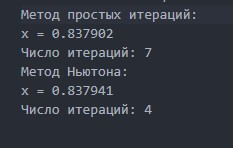
\includegraphics[width=.9\textwidth]{img1}
\caption{Входные данные}
\end{figure}
% \pagebreak

\subsection{Результаты работы}
\begin{figure}[h!]
\centering
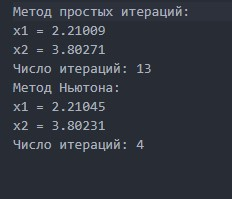
\includegraphics[width=.9\textwidth]{img2}
\caption{Вывод программы в консоли}
\end{figure}
В процессе решения задачи выяснилось,что точное решение,заданное в условиях задачи,не корректно
% \vfill

% \begin{figure}[h!]
% \centering
% \includegraphics[width=.9\textwidth]{lab5_taylor}
% \caption{Решение с аппроксимацией граничных условий со вторым порядком}
% \end{figure}
\pagebreak

\subsection{Исходный код}
% \lstinputlisting[language=C++]{matrix.cpp}
% \begin{lstlisting}
\lstinputlisting{include/4.2.cpp}
% \end{lstlisting}
% \lstinputlisting{matrix.cpp}
% {../../include/matrix.cpp}
% \pagebreak
% \lstinputlisting[title=\texttt{parabolic\_pde.hpp}]{../../include/partial_differential/parabolic_pde.hpp}
% \pagebreak
% 